\documentclass[10pt]{article}
\usepackage[paperheight=29.7cm,paperwidth=21cm,outer=1.5cm,inner=1.5cm,top=2cm,bottom=2cm]{geometry}
\usepackage{amsthm, amssymb, amsfonts, amsmath}
\usepackage{graphicx}
\usepackage{wrapfig}
\usepackage{multicol}
\usepackage{tikz}
\usepackage{subfig}
\usetikzlibrary{calc,shapes}
\usepackage{enumitem}
\usepackage{float}
\usepackage{mathtools}
\usepackage{mathrsfs}
\usepackage{tikz-cd}
\usepackage{hyperref, mathabx}
\usepackage{makecell}

\newcommand{\boxitem}[2]{\vspace{.55cm}
\item[#1]
\leavevmode
\strut
\vadjust{%%
\noindent
\raisebox{\dimexpr\dp\strutbox+\ht\strutbox+1ex}[0pt][0pt]{\tikzmark{bl}}}%%
#2
\leavevmode
\vadjust{%
\noindent
\hspace*{\dimexpr\textwidth+1ex}\tikzmark{br}}%%

\tikz[overlay,remember picture]{\draw[black]
(bl) rectangle
(br);}}

\newcommand{\tikzmark}[1]{\tikz[overlay,remember picture] \node (#1) {};}

\newcommand{\C}{\mathbb{C}}
\newcommand{\R}{\mathbb{R}}
\newcommand{\Q}{\mathbb{Q}}
\newcommand{\Z}{\mathbb{Z}}
\newcommand{\N}{\mathbb{N}}
\newcommand{\p}{\mathbb{P}}
\newcommand{\E}{\mathbb{E}}
\newtheorem*{lemma}{Lemma}
\newtheorem{llemma}{Lemma}
\newtheorem*{theorem}{Theorem}
\newtheorem*{prop}{Proposition}


\title{\Huge \textbf{Molecular Physics solved exercises}}

\author{
  Giacomo Fantoni\qquad\qquad\qquad\qquad\quad
  \small Telegram: \href{https://t.me/GiacomoFantoni}{@GiacomoFantoni} \\[3pt]
  Ilaria Cherchi\qquad\qquad\qquad\qquad\quad
  \small Telegram: \href{https://t.me/ilariacherchi}{@ilariacherchi} \\[3pt]
  Alessia Guadagnin Pattaro\qquad
  \small Telegram: \href{https://t.me/alessiagp}{@alessiagp} \\[3pt]
  Elisa Pettin\`a\qquad\qquad\qquad\qquad\quad
  \small Telegram: \href{https://t.me/elisapettina}{@elispettina} \\[3pt]
  Stefano Cretti\qquad\qquad\qquad\qquad\quad
  \small Telegram: \href{https://t.me/StefanoCretti}{@StefanoCretti} \\[3pt]
\small Github: \href{https://github.com/giacThePhantom/MolecularPhysics}{https://github.com/giacThePhantom/MolecularPhysics}}

\begin{document}
  \maketitle
  \tableofcontents
  \graphicspath{{solved_exercises/exercises_images/}}

  \section{Partial derivatives}

  \subsection{Solving partial derivatives}
  Compute all first order partial derivatives of $f(x, y, z) = ze^{-x^2-y^2}$.
  \begin{align*}
    \frac{\partial f}{\partial x} & = -2xze^{-x^2-y^2} \\
    \frac{\partial f}{\partial y} & = -2yze^{-x^2-y^2} \\
    \frac{\partial f}{\partial z} & = e^{-x^2-y^2}\\
  \end{align*}

  Compute both first order partial derivatives of $f = e^{ix}(x^3 + y^3 + 1)$.
  \begin{align*}
    \frac{\partial f}{\partial x} & = ie^{ix}(x^3 + y^3 + 1) + e^{ix}(3x^2) \\
                                  & = e^{ix}(ix^3 + iy^3 + i + 3x^2) \\
    \frac{\partial f}{\partial y} & = 3y^2e^{ix} \\
  \end{align*}

  Compute $\frac{\partial^5f}{\partial^2x\partial^3y}$ with $f = xy^3e^{-\frac{1}{y}} + 5e^{ix^3}y^2$.
  \begin{align*}
    f                                           & = xy^3e^{-\frac{1}{y}} + 5e^{ix^3}y^2 \\
    \frac{\partial f}{\partial x}               & = y^3e^{-\frac{1}{y}} + i15x^2e^{ix^3}y^2\\
    \frac{\partial^2f}{\partial^2x}             & = i15y^2[(2x)(e^{ix^3}) + (x^2)(i3x^2e^{ix^3})]\\
                                                & = i15y^2xe^{ix^3}(2 + i3x^3)\\
    \frac{\partial^3f}{\partial^2x\partial y}   & = i30yxe^{ix^3}(2 + i3x^3) \\
    \frac{\partial^4f}{\partial^2x\partial^2y}  & = i30xe^{ix^3}(2 + i3x^3) \\
    \frac{\partial^5f}{\partial^2x\partial^3y}  & = 0 \\
  \end{align*}

  % TODO Add exercises on differential equations

  \section{Differential operators}

  \subsection{Computing the gradient of a function}
  Compute $\text{grad}(f)$ with $f = x^2 + y^2 + z^2$.
  \begin{align*}
    \text{grad}(f) = \vec\nabla f
      & = \begin{pmatrix}
            \frac{\partial f}{\partial x} &
            \frac{\partial f}{\partial y} &
            \frac{\partial f}{\partial z}
          \end{pmatrix} \\
      & = \begin{pmatrix}
            2x & 2y & 2z
          \end{pmatrix}
  \end{align*}
  % TODO Normalize result

  Compute $\text{grad}(f)$ with $f = \sin(x^2yz)$.
  \begin{align*}
    \text{grad}(f) = \vec\nabla f
      & = \begin{pmatrix}
            \frac{\partial f}{\partial x} &
            \frac{\partial f}{\partial y} &
            \frac{\partial f}{\partial z}
          \end{pmatrix} \\
      & = \begin{pmatrix}
            xyz\cos(x^2yx) &
            x^2z\cos(x^2yx) &
            x^2y\cos(x^2yx)
          \end{pmatrix}
  \end{align*}

  \subsection{Computing the divergence of a function}
  Compute $\text{div}(\vec f \,)$ with $\vec f = \begin{pmatrix} xy & y & zx^2\end{pmatrix}$.
  \begin{align*}
    \text{div}(\vec f \,) = \vec\nabla \cdot \vec f
      & =
        \begin{pmatrix}
          \frac{\partial}{\partial x} &
          \frac{\partial}{\partial y} &
          \frac{\partial}{\partial z}
        \end{pmatrix} \cdot
        \begin{pmatrix}
          f_x & f_y & f_z
        \end{pmatrix} \\
      & =
        \frac{\partial f_x}{\partial x} +
        \frac{\partial f_y}{\partial y} +
        \frac{\partial f_z}{\partial z} \\
      & =
        \frac{\partial (xy)}{\partial x} +
        \frac{\partial (y)}{\partial y} +
        \frac{\partial (zx^2)}{\partial z} \\
      & = y + 1 + x^2 \\
  \end{align*}

  \subsection{Computing the curl of a function}
  Compute $\text{rot}(\vec f \,)$ with $\vec f = \begin{pmatrix} y & -x & 0\end{pmatrix}$.
  \begin{align*}
    \text{rot}(\vec f \,) = \vec\nabla \times \vec f
      & =
        \begin{pmatrix}
          \frac{\partial f_z}{\partial y} - \frac{\partial f_y}{\partial z} &
          \frac{\partial f_x}{\partial z} - \frac{\partial f_z}{\partial x} &
          \frac{\partial f_y}{\partial x} - \frac{\partial f_x}{\partial y}
        \end{pmatrix} \\
      & =
        \begin{pmatrix}
          \frac{\partial (0)}{\partial y} - \frac{\partial (-x)}{\partial z} &
          \frac{\partial (y)}{\partial z} - \frac{\partial (0)}{\partial x} &
          \frac{\partial (-x)}{\partial x} - \frac{\partial (y)}{\partial y}
        \end{pmatrix} \\
      & =
        \begin{pmatrix}
          0 - 0 & 0 - 0 & -1 - -1
        \end{pmatrix} \\
      & =
        \begin{pmatrix}
          0 & 0 & -2
        \end{pmatrix} \\
  \end{align*}
  % TODO Standardize?

  \subsection{Curl of the grad of a function}
  Compute $\text{rot}(\text{grad}(\vec f))$.

  \begin{align*}
  \text{rot}(\text{grad}(\vec f \,)) = \vec\nabla \times \left(\vec\nabla \vec f\,\right)
    & =
      \vec\nabla \times
      \begin{pmatrix}
        \frac{\partial f}{\partial x} &
        \frac{\partial f}{\partial y} &
        \frac{\partial f}{\partial z}
      \end{pmatrix} \\
    & = \det
      \begin{vmatrix}
        \vec e_x & \vec e_y & \vec e_z \\[6pt]
        \frac{\partial}{\partial x} &
        \frac{\partial}{\partial y} &
        \frac{\partial}{\partial z} \\[6pt]
        \frac{\partial f}{\partial x} &
        \frac{\partial f}{\partial y} &
        \frac{\partial f}{\partial z}
      \end{vmatrix} \\
    & =
      \begin{pmatrix}
        \frac{\partial^2 f}{\partial y \partial z} - \frac{\partial^2 f}{\partial z \partial y} &
        \frac{\partial^2 f}{\partial z \partial x} - \frac{\partial^2 f}{\partial x \partial z} &
        \frac{\partial^2 f}{\partial x \partial y} - \frac{\partial^2 f}{\partial y \partial x}
      \end{pmatrix} \\
    & \text{since you can change the order of derivation} \\
    & =
      \begin{pmatrix}
        0 & 0 & 0
      \end{pmatrix}
  \end{align*}
  Notice that $\text{rot}(\text{grad}(\vec f))$ is equal to the zero vector regardless of $f$.

  \subsection{Divergence of the curl of a function}
  Compute $\text{div}(\text{rot}(\vec f))$.

  \begin{align*}
  \text{div}(\text{rot}(\vec f \,)) = \vec\nabla \cdot \left(\vec\nabla \times \vec f\,\right)
    & =
      \vec\nabla \cdot
      \begin{pmatrix}
        \frac{\partial f_z}{\partial y} - \frac{\partial f_y}{\partial z} &
        \frac{\partial f_x}{\partial z} - \frac{\partial f_z}{\partial x} &
        \frac{\partial f_y}{\partial x} - \frac{\partial f_x}{\partial y}
      \end{pmatrix} \\
    & =
      \begin{pmatrix}
        \frac{\partial f}{\partial x} &
        \frac{\partial f}{\partial y} &
        \frac{\partial f}{\partial z}
      \end{pmatrix}
      \cdot
      \begin{pmatrix}
        \frac{\partial f_z}{\partial y} - \frac{\partial f_y}{\partial z} &
        \frac{\partial f_x}{\partial z} - \frac{\partial f_z}{\partial x} &
        \frac{\partial f_y}{\partial x} - \frac{\partial f_x}{\partial y}
      \end{pmatrix} \\
    & =
      \frac{\partial^2 f_z}{\partial y \partial x} - \frac{\partial^2 f_y}{\partial z \partial x} +
      \frac{\partial^2 f_x}{\partial z \partial y} - \frac{\partial^2 f_z}{\partial x \partial y} +
      \frac{\partial^2 f_y}{\partial x \partial z} - \frac{\partial^2 f_x}{\partial y \partial z} \\
    & \text{then, changing the order of the terms we notice that} \\
    & =
      \frac{\partial^2 f_z}{\partial y \partial x} - \frac{\partial^2 f_z}{\partial x \partial y} +
      \frac{\partial^2 f_x}{\partial z \partial y} - \frac{\partial^2 f_x}{\partial y \partial z} +
      \frac{\partial^2 f_y}{\partial x \partial z} - \frac{\partial^2 f_y}{\partial z \partial x} \\
    & \text{since you can change the order of derivation} \\
    & = 0
  \end{align*}
  Notice that $\text{div}(\text{rot}(\vec f))$ is equal to zero vector regardless of $f$.

  \subsection{Divergence of the gradient of a function}
  Demonstrate that $\Delta f = \text{div}(\text{grad}(f))$

  \begin{align*}
  \text{div}(\text{grad}(\vec f\,)) = \vec\nabla \cdot \left(\vec\nabla \vec f\,\right)
    & =
      \vec\nabla \cdot
      \begin{pmatrix}
        \frac{\partial f}{\partial x} &
        \frac{\partial f}{\partial y} &
        \frac{\partial f}{\partial z}
      \end{pmatrix} \\
    & =
      \begin{pmatrix}
        \frac{\partial}{\partial x} &
        \frac{\partial}{\partial y} &
        \frac{\partial}{\partial z}
      \end{pmatrix}
      \cdot
      \begin{pmatrix}
        \frac{\partial f}{\partial x} &
        \frac{\partial f}{\partial y} &
        \frac{\partial f}{\partial z}
      \end{pmatrix} \\
    & =
      \frac{\partial^2 f}{\partial^2 x} +
      \frac{\partial^2 f}{\partial^2 y} +
      \frac{\partial^2 f}{\partial^2 z} \\
    & = f
      \left(
      \frac{\partial^2}{\partial^2 x} +
      \frac{\partial^2}{\partial^2 y} +
      \frac{\partial^2}{\partial^2 z}
      \right) \\
    & = \Delta f
  \end{align*}

  \section{Spherical coordinates}
  % TODO
  \section{Multidimensional integrals}

  \subsection{Computing multidimensional integrals}
  Compute $\int\limits_{y=0}^{y=\pi}\int\limits_{x=y}^{x=\pi}\frac{sinx}{x}dxdy$.
  \begin{align*}
    \int\limits_{y=0}^{y=\pi}\int\limits_{x=y}^{x=\pi}\frac{sinx}{x}dxdy
      & = \int\limits_{x=0}^{x=\pi}\int\limits_{y=0}^{y=x}\frac{sinx}{x}dydx
      & \text{change order of integration}\\
      & = \int\limits_{x=0}^{x=\pi} \left[y\frac{sinx}{x}\right]_{y=0}^{y=x}dx
      & \text{integrate over y} \\
      & = \int\limits_{x=0}^{x=\pi} \left(x\frac{sinx}{x} - 0\frac{sinx}{x}\right)dx
      & \text{evaluate over interval of y} \\
      & = \int\limits_{x=0}^{x=\pi} \sin x \, dx
      & \text{simplify} \\
      & = [-\cos x]_{x=0}^{x=\pi}
      & \text{integrate over x} \\
      & = (-\cos\pi-\cos0)
      & \text{evaluate over interval of x} \\
      & = - (-1) - (-1) = 2 \\
  \end{align*}

  Notice how the integration region changes when swapping order of integration. To understand how the integration region changes, look at \ref{fig:integration_area}.
  \begin{figure}[h]
    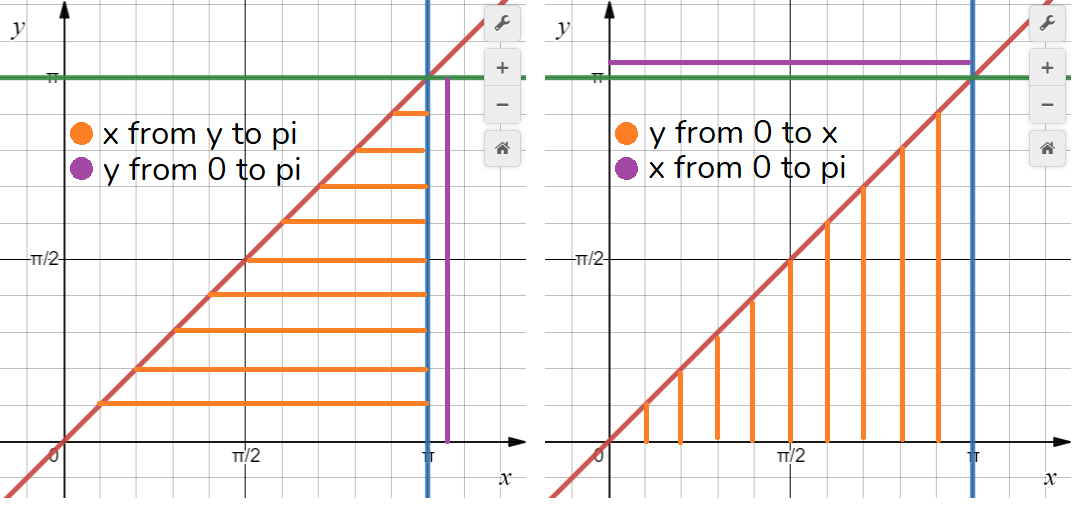
\includegraphics[width=\textwidth]{integration_area.png}
    \caption{On the left: original order of integration. On the right: inverted order of integration}
    \label{fig:integration_area}
  \end{figure}

  \section{Wave equations}
  % TODO
  \section{Hilbert spaces}
  % TODO
\end{document}
